% Brian Cain
% CIS 751 Computer and Information Security
% Final Report
% Due December 7th, 2012

% TEMPLATE for Usenix papers, specifically to meet requirements of
%  USENIX '05
% originally a template for producing IEEE-format articles using LaTeX.
%   written by Matthew Ward, CS Department, Worcester Polytechnic Institute.
% adapted by David Beazley for his excellent SWIG paper in Proceedings,
%   Tcl 96
% turned into a smartass generic template by De Clarke, with thanks to
%   both the above pioneers
% use at your own risk.  Complaints to /dev/null.
% make it two column with no page numbering, default is 10 point

% Munged by Fred Douglis <douglis@research.att.com> 10/97 to separate
% the .sty file from the LaTeX source template, so that people can
% more easily include the .sty file into an existing document.  Also
% changed to more closely follow the style guidelines as represented
% by the Word sample file. 

% Note that since 2010, USENIX does not require endnotes. If you want
% foot of page notes, don't include the endnotes package in the 
% usepackage command, below.

% This version uses the latex2e styles, not the very ancient 2.09 stuff.
\documentclass[letterpaper,twocolumn,11pt]{article}
\usepackage{datetime,usenix,epsfig,graphicx}
\begin{document}

%don't want date printed
\date{}

%make title bold and 14 pt font (Latex default is non-bold, 16 pt)
\title{\Large \bf Threat of malicious hardware trojans}

%for single author (just remove % characters)
\author{
{\rm Brian Cain}\\
Department of Computer Science\\
Kansas State University\\
bccain@ksu.edu
% copy the following lines to add more authors
% \and
% {\rm Name}\\
%Name Institution
} % end author

\maketitle

% Use the following at camera-ready time to suppress page numbers.
% Comment it out when you first submit the paper for review.
\thispagestyle{empty}

\begin{abstract}
{\em Hidden malicious circuits can provide a backdoor for attackers to compromise computer systems without the knowledge of the user. These hardware trojans (HT) can sit on the hardware layer of a computer system and bypass any software or anti-virus that a user may have. Some of these attacks include built-in backdoors, privilege escalation, and password stealing. Unfortunately without completely tearing down the entire logic circuit (thus rendering it useless), it is very difficult to determine if hardware has a hidden trojan installed. A research group from the University of Illinois Urbana has shown that integrated logic circuits can be designed, created, and used with hidden malicious intent. There has also been some advanced research in detecting and preventing HTs on logic circuits. This paper will go through these research papers and discuss the results found from the current research in the field of creating and detecting malicious hardware trojans.}
\end{abstract}
\section{Introduction}
\subsection{Background}
A hardware trojan (HT) is known to be a malicious design of an integrated circuit. While the purpose of a software trojan is to grant someone with unauthorized access to a computer on the software level, a HT can do the same through the hardware level. If a HT is successfully implanted into a machine, there is a potential for malicious activity such as backdoor access, along with passwords from a shadow file becoming compromised. \\

Some of these attacks have already been implemented using a custom made integrated circuit~\cite {king}. This specific design was implemented by The University of Illinois Champaign. When the design and manufacturing process of integrated circuits was majorly based in the United States, it was easier to keep track of what was going on. However, now this process has been outsourced overseas into different parts of the world~\cite {wei, teh}. Because of this, the authenticity of a chip is difficult to verify with 100\% assurance without taking the integrated circuit apart rendering it unusable.\\

Another problem with the manufacturing process moving overseas is that the entire design process is often done in untrusted factories~\cite {teh}. This means that if a fabrication factory is untrusted, an adversary could be able to alter the design of the integrated circuits and place a hidden malicious HT into the design. Because of this potential for an attack, techniques have been proposed to detect HT that does not render the integrated circuit unusable.

\subsection{Similar Attacks}
King et al.\ ~\cite {king} explain a few attacks from the past that are similar to HT's. Attacks similar to HT have already been made a reality through a few different products. For example, in 2006 Apple released iPod videos that were infected with a trojan called RavMonE. The trojan infected windows computers by modifying the windows registry, then it opened a random port on the computer to accept commands remotely. Another attack similar to a HT that happened recently was found on Seagate external hard drives from Taiwan. These external hard drives had a trojan shipped with it that sent personal data to a remote attacker \cite {king}. These attacks have a similar idea to a HT in that you expect to buy a product from a trusted manufacturer, only to have the device compromised. 

\subsection{Threat Model}
Motivated attackers can subvert the integrated circuit supply chain, change the designs of a given processor, and get it on the production line. In other words, this type of attack is not open to everyone. It will require a design change that top level, and it must make it through any sort of design analysis at a large foundry~\cite {teh}. So this is an expensive attack and requires some sort of higher level of privilege access. Your average script kiddy will most likely not be able to perform a successful HT attack. However, larger organizations such as government agencies, crime groups, terrorist groups have the means to perform an attack such as this. 

\section{Classification}
There are three main ways we can classify HT's. Although many of them have the same goal, they all can function in different ways. According to Tehranipoor et al.\ ,``\ldots the industry lacks metrics to evaluate the effectiveness of methods in detecting Trojans''~\cite {teh}. Because of this, they have attempted to classify different HT's into three main categories relating to their physical, activation, and action characteristics (See Figure~\ref{tax} for a more visual description). The next few sections detail these different characteristics.

\begin{figure}[ht!]
\centering
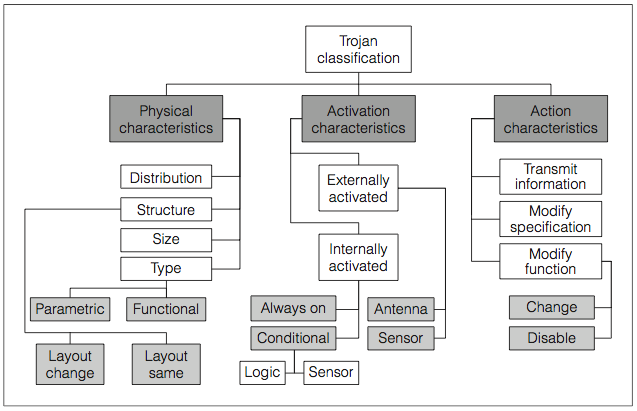
\includegraphics[width=80mm]{images/tax.png}
\caption{The three main classifications of hardware trojans are: Physical Characteristics, Activation Characteristics, and Action characteristics. (Source: Tehranipoor et al.~\cite {teh})}
\label{tax}
\end{figure}

\subsection{Physical Characteristics}
The physical characteristics of a HT describe the different kinds of hardware manifestations. The distribution category classifies the actual location of a potential HT on a integrated circuit. The structure category splits up into two possible options: Layout Change and Layout Same. These differences are basically either the HT changes the layout of a given integrated circuit, or keeps it the same. This is important because if there is a chance in the integrated circuit, then this could completely change the chips delay and power characteristics, thus making trojan detection easier if the layout is changed. Next we have size, which refers to the number of components in the chip that were added, deleted or compromised by the HT. Finally we have the type of physical characteristics. This can be broken down into either functional which means the trojans are created through the addition or deletion of transistors or gates on the integrated circuit. The second part of type classification is parametric, which means the HT is created through the modification of existing wires and logic.

\subsection{Activation Characteristics}
The activation characteristics are about the different ways that a HT can be activated after installed in a machine. There are two major ways that HT can be activated. The first one is externally. This can be done with an antenna or a sensor that can interact from the outside of the machine. To minimize the HT's detectability, you would not want the HT always on, otherwise it would give away that the chip was compromised (through chip delay and power characteristics). So if you an attacker, a chip that was activated remotely would be ideal. The second way that a HT can be activated is internally. The two ways this can happen is either to be always on (but this can increase detectability as detailed in King et al\.'s paper~\cite {king}). The second way a chip could be activated internally is by inserting a trojan at a path in the chip that are rarely used. Then through some sort of packet or electronic pulse sent to the specific part on the logic board, the HT will be activated. The second case is very difficult to detect.

\subsection{Action Characteristics}
The action characteristics classify the different types of way the trojan can behave. This section is divided up into three types of attacks: transmitting information, modify specification, and modify function. The transmit information section is an action where a trojan can send important or secret information to an adversary. Modify specification means when a trojan attacks the chips parametric properties, like modifying existing wire and transistor geometries. Finally, the modify function refers to when a trojan can bypass the chips existing logic.

\section{Illinois Malicious Processor}
\subsection{Design}
King et al.\ ~\cite {king} has designed and implemented a malicious piece of hardware much like the ones described in the previous section. This proof of concept design was successfully created by the University of Illinois at Urbana Champaign, and it was named Illinois Malicious Processors (IMPs). 

\subsection{Kinds of Attacks}
With the IMP, King et al.\ ~\cite {king} has shown three powerful attacks through two different kinds of HT. Through the modification of the CPU, they consider two main malicious ways to attack. The {\em memory access} modification gives the attacker the ability to go around the OS's isolation expectations, such as privilege escalation. The {\em shadow mode} allows the hidden execution of different kinds of hardware attacks, such as a backdoor to allow an attacker to login with, or even password stealing. Both of these modifications use a minimal number of transistors making it semi-difficult to detect, and both are powerful attacks.

\subsection{Memory Access}
The memory access modification of a CPU provides support for unprivileged malicious software to access privileged memory regions on the compromised machine. Simply, this is accomplished by loading a {\em magic value} on the data bus, which will then disable any sort of checking by the host OS. Once this value is loaded into the memory bus, malicious software triggers the attack so that the memory access circuits become enabled. Once this sequence has been triggered, the memory management unit (MMU) in the data cache ignores any CPU privilege levels for memory access. This now grants unprivileged software access to all memory on the host OS, including regions of memory that are reserved for the OS's internal memory. This attack only adds 959 logic gates to a baseline processor, or about 0.05\% overall. This is a very small attack, and the percentage will be even smaller as integrated circuits become more advanced. \\

With memory access, you can perform a privilege escalation attack on the compromised host OS. This malicious service escalates the user process to root privilege. To perform this attack, a malicious piece of software enables the memory access CPU modification to turn off protection of any memory region. While this is off, it finds the user process in the kernel memory and changes its user ID to root. This is all accomplished without any sort of software bug or exploit.

\subsection{Shadow Mode}
\begin{figure}[ht!]
\centering
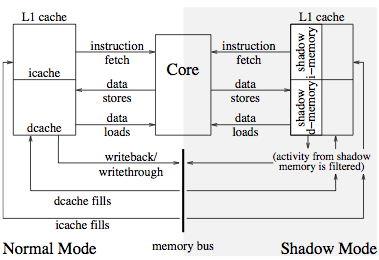
\includegraphics[width=80mm]{images/shadow.png}
\caption{How the hardware differs while shadow mode is enabled. (Source: King et al.~\cite {king})}
\label{shadow}
\end{figure}

Shadow mode has been implemented by reusing existing circuits. It accomplishes this by executing instructions invisible to the hardware outside of the IMP. Not only is this undetectable by the hardware, but it is also undetectable by the software. Figure~\ref{shadow} shows the difference between running in normal mode and shadow mode. In normal mode, it operates like a regular integrated circuit. In shadow mode however, the process is able to limit what activity will go out to the memory bus. This attack only adds 1341 logic gates, for a total of 0.08\% overall to a baseline processor. This also adds 117 lines of code. Loading up shadow mode attacks onto the IMP requires two main bootstrap mechanisms. \\

The first bootstrap mechanism is to initialize the attack by including a small section of bootstrap code in the cache memory. This code can be made up of ``normal CPU instructions that are executed after a processor reset''~\cite {king}. The second bootstrap mechanism is known as a bootstrap trigger. This trigger tells the IMP to load in a firmware from nearby data. This can be easily accomplished if the host OS is connected to the internet with a network interface. When the host OS is connected to the internet, an attacker can send a random packet to the OS for it to drop. Even if the packet contains arbitrary information, the OS still must inspect the packet being sent before it can drop it. Shadow mode uses this idea to activate its bootstrap trigger. In other words, the act of inspecting the arbitrary packet to drop provides a sufficient opportunity to start the trigger. Once it gets this packet, it can silently load the data within the dropped packet in shadow mode, again making it invisible to the hardware and software. If the computer is not connected to a network interface, this can be accomplished by using a thumb drive. \\

There are a couple of very powerful attacks that can be accomplished by using shadow mode. The first one is a backdoor login system. Once shadow mode is activated through the network interface or a usb, the hidden firmware detects when a user tries to login with the password ``letmein''. This malicious firmware forces the password checking function to return true, and then the attacker is granted access. Finally to avoid detection, the shadow mode firmware detaches itself after the attacker logs in.  \\

The second attack that can be accomplished by shadow mode is password stealing. The shadow mode firmware uses the write library call from the OS to search for a string ``Password:'' to identify any processes that receive passwords from a user. The on the following read call, it moves in between library calls to steal potential passwords on the system. Once shadow mode successfully compromises passwords, it attempts to send the stolen passwords by interacting with the OS network. One potential way shadow mode can do this is by overwriting existing network frames with shadow modes own UDP packets. These malicious packets contain a predetermined IP address to return to, along with the stolen password data. A problem with this attack however is when shadow mode attempts to interact with the host OS network interface, it can make itself visible and thus easier detected.

\subsection{Research Results}
Once IMP was designed and implemented, King et al.\ ~\cite {king} did a number of timing perturbation tests comparing the IMP against a baseline processor. Figure~\ref{kingtiming} shows the different comparisons made while running a few different process benchmarks: gcc, parser, twolf, bzip2, wget, and AVG. According to their results, the IMP does not affect or change the timing of the processor. The experiment consisted of four different cases: {\bf Baseline} is when all of the processes run with unmodified hardware and does not attack. {\bf Known Root} is run on unmodified hardware, and the attack is accomplished through a known root password. With the known root, they steal the /etc/shadow file. {\bf Transient} is when the benchmarks are run on hardware with shadowmode support. They used a hardware login backdoor to steal the /etc/shadow file. {\bf Persistent} is when shadow mode is never disabled, and the login backdoor is used. This is a much larger overhead compared to the other attacks. \\

Overall, both the memory access and shadow mode modifications require very little logic gates, and only add a total of 0.13\% addition to a baseline processor. As mentioned before and in the paper, as integrated circuits become more complicated over the years, this percentage will shrink, making it more difficult to detect. Even with the small amount of logic gates, the IMP allows the adversary to execute high-level attacks to the host OS. 

\begin{figure}[ht!]
\centering
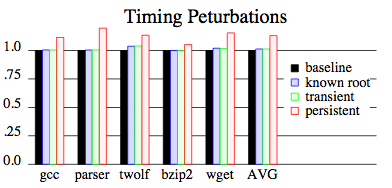
\includegraphics[width=85mm]{images/timing_king.png}
\caption{Timing Peturbations observed compare the Illinois Malicious Processor against a non-attack circuit. (Source: King et al.~\cite {king})}
\label{kingtiming}
\end{figure}

\section{Detection}
Hardware designs of integrated circuits are rather complicated, and as proven by King et al., a successful HT only needs a small percentage of modifications to accomplish an attack. To detect these HT's physically, you end up destroying the chip, thus rendering it unusable. Some HT's are activated with specific conditions (such as the network packet in IMP), however it is rather unlikely to find the specific conditions to activate the HT from random stimuli~\cite {teh}. \\

Another issue with HT detection is that HT can be hidden within flucuations due to process variation on a processor, so its impact on differing from a baseline processor is too small to be detected by modern instruments~\cite {wei}. Even with these detection issues present, Tehranipoor et al. and Wei et al. have proposed a few techniques for detecting HT's on potentially compromised integrated circuits. 

\subsection{Side-Channel Signal Analysis}
This type of analysis is when you observe timing and power of a potential malicious circuit, and was proposed by Argawal et al.~\cite {arg}. This style of analysis can help detect a HT without destroying the integrated circuit. If you have an instrument that is very sensitive to the flucuations in power and timing, then you can compare a potentially malicious integrated circuit against a baseline processor. The HT will differ from the baseline version. \\

{\em Power-based} side channel signal analysis is accomplished by first analyzing the baseline integrated processor. Random patterns and power measurements are performed all across the processor to get a base test of data. Once this data is obtained, the same measurements are performed on the potentially malicious integrated circuits to see if there are any major differences. If the trojan is large enough, the difference will be easily discovered. However Wei et al. show how it's possible to create HT's that have the ability to mask their power flucuations~\cite {wei}. The downside to this type of detection according to Tehranipoor et al. is that the ``amount of current a {\em (HT)} can draw might be so small that it could be submerged into an envelope of noise and process variation effects, and thus be undetectable by conventional measurement equipment''~\cite {teh}. In other words, there might be so much already going on with a complex integrated circuit that the smaller HT might be almost completely overshadowed by the more complex circuitry. \\ 

{\em Timing-based} side channel signal analysis is accomplished by using a sweeping-clock-delay measurement technique to measure selected register-to-register path delays. In simplier terms, this technique aims to discover hidden circuity such as a shadow register by testing the timing of a potential malicious integrated circuit against a baseline circuit. These timing features that are being measured generate a specific path delay fingerprint ~\cite {teh}. Because of this, it doesn't matter how small the HT is on the chip, because if one is present on a potentially malicious integrated circuit the fingerprint path will differ from a baseline circuit's fingerprint. While this method can be effective in the detection of HT's, the modern circuits of today can include millions of paths. This means measuring all of these paths for every individual circuit is not very practical~\cite {teh}. 

\subsection{Trojan Activation}
Trojan activation analysis attempts to enable a HT through random stimuli on the potentially malicious integrated circuit. If some part of the malicious piece of hardware is activated, the HT is likely to consume more power than a baseline circuit. This then gives us a methodology for detecting HT's by activation. These strategies, if done right, can accelerate the Trojan detection process. Often times these techniques are used along side power analysis techniques for an effective way of discovering HT's. \\

This sort of rare activation trigger is shown in a diagram found at Figure~\ref{activation}. First you see the primary input section of the model, which can be anything. Those primary inputs, if correct, can in turn trigger either q1 or q2. Once this occurs, the Trojan circuit is activated and the payload is executed. Usually however, q1 and q2 are very difficult to discover, making trojan activation detection analysis a very difficult process. Despite this, there are two different kinds of trojan activation techniques that can be used. \\

\begin{figure}[ht!]
\centering
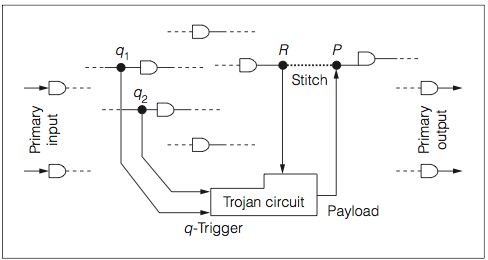
\includegraphics[width=80mm]{images/act.png}
\caption{A hardware trojan circuit model that shows a trigger activation condition. (Source: Tehranipoor et al. ~\cite {teh})}
\label{activation}
\end{figure}

{\em Region-free} trojan activation techniques do not focus on any specific region of an intergrated circuit. It applies input patterns to the entire suspicious integrated circuit and comares it to the baseline circuit. This style of methodology ``{\em (relies)} on the accidental or systematic activation of trojans''~\cite {teh}. This method reliies on the fact that the original design of the chip and the chip being tested are the same. If there is any difference in the design, even not malicious, differences will be present and might give false results. \\

{\em Region-aware} trojan activation techniques apply input patterns and increase activity to specific portions of the circuit while the rest is simultaneously decreased. Again, these results are mirrored on a baseline circuits to measure any differences. This style of methodology is also known as circuit partitioning and activity magnification. \\

Because it's impossible to know the size of type of the trojan, testing will require both region-free and region-aware trojan activation detection techniques. For example, if a HT trigger depends on the random inputs of various sections of the integrated circuit, the region-free testing would be required. However if the HT depends on triggers that are dependant on a specific region, then region-aware testing will be needed.

\subsection{Architecture-level Trojan Detection}
The idea behind this is to authenticate hardware by checking details at a lower level. This includes using a checksum based on cycle-to-cycle activities. Once you obtained this checksum, you could compare your potentially malicious HT against a baseline processor. However the problem with this is if your baseline processor is also some how compromised at the design level, then you still can't be assured that your potentially malicious integrated circuit is actually safe or not. However it is an interesting idea if your baseline source is coming from a trusted manufacurer.

\subsection{Mitigation of Information Leakage}
Das et al.~\cite {das} explain an approach to detect and prevent information leakage such as the password stealing attack detailed in the IMP shadow mode password stealing attack. They claim that information leakage often take place due to illegal writes to the main memory. They propose a way to detect this sort of attack with an external guardian, seperate from the host hardware, that will have to approve each memory request. \\

This sort of mitigation might be able to preven the memory access attack shown by the IMP. For example, if the MMU is altered to allow the IMP to give an adversary a root ID, that call would have to be approved by the external guardian even if IMP turns off all privilege checks for the host processor. Because the guardian and the host machine are seperate, the guaridian must be compromised for a memory access attack to succede.

\section{Conclusions}
We have shown that hardware trojans are possible to design and implement as demonstrated by the University of Illinois at Urbana Champaign called the Illinois Malicious Processor. These hardware trojans can successfully execute their payloads and accomplish such attacks as privilege escalation, backdoor logins, and password stealing. These attacks, while complicated and powerful, surprisingly add a very small amount of logic gates to the baseline processor. This makes hardware trojans very difficult to detect, especially when integrated circuits are becoming more compliated. \\

Mitigation detection for hardware trojans include side-channel analysis, trojan activation, architecture level trojan detection, and prevention of information leakage. These detection and prevention techniques provide some hope for discovering real hardware trojans in the wild. \\

It is important to remember that attacks such as hardware trojans start at a compromised foundry, and cannot be done by the average adversary. This often involves changing the original baseline design of the integrated processor, and getting past any checks for validation of the designs. A way to help prevent this sort of adversary attack is to put strict requirements and specifications for integrated circuit design and manufacturing in these foundries not located in the United States. Again, because it is not a trivial or inexpensive task to create your own integrated circuit, we must rely on the foundaries over seas. If we continue to want to do business with these companies, we must make sure that these requirements are followed. \\

Because of how expensive and how complicated these attacks are, they are most likely not currently targeted at the average user. Motivated Attackers will create their own custom integrated circuits if the attacks are worth the effort, despite the cost. Government organizations, crime groups, terrorist groups, ect all have the funds to produce such attacks. Overall, hardware trojans are a very powerful attack, and more research should be done in this area for the prevention and detection of hardware circuits. \\

\begin{thebibliography}{1}

  \bibitem{das} Abhishek Das, Gokhan Memik, Joseph Zambreno, and Alok Choudhary. 2010. Detecting/preventing information leakage on the memory bus due to malicious hardware. In {\em Proceedings of the Conference on Design, Automation and Test in Europe} (DATE '10). European Design and Automation Association, 3001 Leuven, Belgium, Belgium, 861-866.

  \bibitem{arg} D. Agrawal et al., ‘‘Trojan Detection Using IC Fingerprinting,’’ Proc. IEEE Symp. Security and Privacy (SP 07), IEEE CS Press, 2007, pp. 296-310.

  \bibitem{teh} Mohammad Tehranipoor and Farinaz Koushanfar. 2010. A Survey of Hardware Trojan Taxonomy and Detection. {\em IEEE Des.} Test 27, 1 (January 2010), 10-25. DOI=10.1109/MDT.2010.7 http://dx.doi.org/10.1109/MDT.2010.7

  \bibitem{king} Samuel T. King, Joseph Tucek, Anthony Cozzie, Chris Grier, Weihang Jiang, and Yuanyuan Zhou. 2008. Designing and implementing malicious hardware. In {\em Proceedings of the 1st Usenix Workshop on Large-Scale Exploits and Emergent Threats} (LEET'08), Fabian Monrose (Ed.). USENIX Association, Berkeley, CA, USA, , Article 5 , 8 pages.

  \bibitem{wei} Sheng Wei, Kai Li, Farinaz Koushanfar, and Miodrag Potkonjak. 2012. Hardware Trojan horse benchmark via optimal creation and placement of malicious circuitry. In {\em Proceedings of the 49th Annual Design Automation Conference} (DAC '12). ACM, New York, NY, USA, 90-95. DOI=10.1145/2228360.2228378 http://doi.acm.org/10.1145/2228360.2228378

\end{thebibliography}

\end{document}
